%\documentclass[10pt]{book}
\documentclass[12pt,twoside]{report}
\usepackage[left=2cm,right=2cm,top=2cm,bottom=3cm]{geometry}
\usepackage[utf8]{inputenc}
\usepackage[spanish]{babel}
\usepackage{amsmath}
\usepackage{amsfonts}
\usepackage{amssymb}
\usepackage{float}
\usepackage{graphicx}
\begin{document}

\begin{titlepage}
\begin{center}
\vspace*{-1in}
\begin{figure}[htb]
\begin{center}

\includegraphics[width=8cm]{./logos/cimat.jpg}
\end{center}
\end{figure}
\rule{100mm}{0.2mm}\\
Centro de Investigación en Matemáticas A. C.\\

\begin{Large}
\textbf{ALGORITMOS DE CIFRADO DE DATOS} \\
\end{Large}
\vspace*{0.3in}
\begin{large}
TESIS\\
\end{large}
\vspace*{0.2in}
que para obtener el grado de \\
\vspace*{0.4in}
\begin{large}
Maestría en Ciencias con Especialidad en Computación y Matemáticas Industriales\\
\end{large}
\vspace*{0.2in}
presenta \\
\vspace*{0.4in}
\begin{large}
Marcos Daniel Calderón Calderón\\
\end{large}
\vspace*{0.3in}
Director de Tesis\\
\vspace*{0.2in}
\begin{large}
Rogelio Hasimoto Beltrán\\
\end{large}
\vspace*{0.1in}
\end{center}
\end{titlepage}


%Ahora deseamos agregar una pagina en blanco sin numerar.
%\newpage
%\mbox{}
%\thispagestyle{empty} % para que no se numere esta pagina


%Ahora, vamos a agregar una dedicatoria.
%\chapter*{}
%\pagenumbering{Roman}
%\begin{flushright}
%\textbf{Dedicado a: }

%\textit{Mi familia.}
%\end{flushright}




\chapter{cosas}
\section{Introducción}

Se dice que un mapa $f$ que está definido en el intervalo $I= [\alpha, beta]$ es caótico si se cumplen las siguientes condiciones:

\begin{enumerate}
\item Los puntos periódicos de $f$ son densos en I.
\item $f$ es una función transitiva en el intervalo $I$, esto significa que, dados dos subintervalos cualesquiera $U_{1}$ y $U_{2}$ en $I$, hay un punto $x_{0} \in U_{1}$y un $n>0$ tal que $f^{n}(x_{0} \in U_{2})$.
\end{enumerate}

\chapter{haajad}
\section{Resultados}

Se dice que un mapa $f$ que está definido en el intervalo $I= [\alpha, beta]$ es caótico si se cumplen las siguientes condiciones:

\begin{enumerate}
\item Los puntos periódicos de $f$ son densos en I.
\item $f$ es una función transitiva en el intervalo $I$, esto significa que, dados dos subintervalos cualesquiera $U_{1}$ y $U_{2}$ en $I$, hay un punto $x_{0} \in U_{1}$y un $n>0$ tal que $f^{n}(x_{0}) \in U_{2}$.
\item $f$ tiene dependencia  a las condiciones iniciales en $I$; esto significa que hay una constante de sensibilidad $\beta$ tal que para cualquier $x_{o} \in I$ y cualquier intervalo abierto $U$ sobre $x_{0}$, hay alguna semilla $y_{o} \in U$ Y $n >0$ tal que

\begin{equation}
|f^{n}(x_{0}) - f^{n}(y_{0}) | > \beta.
\end{equation} 
\end{enumerate}

\chapter{Caos Discretizado para la generación de números pseudoaleatorios en Criptografía.}
\section{Introducción}

Los números aleatorios tienen un papel fundamental en Cryptorafía, se utilizan en muchas cosas, por ejemplo, para definir claves de cifrado o contraseñas. Actualemnte, se pueden generar números aleatorios de dos maneras: True Random Number Generators (TGNGs) y Pseudo Random Number Generators (PRNGs). Los primeros son dispositivos que explotan fenómenos físicos un un comportamiento verdaderamente estocástico; por ejemplo, el ruido electróncio de sistemas dinámicos caóticos no lineales, la secuencia obtenida de estos dispositivos tiene un grado intrínseco de impredecibilidad, que es medida mediante las herramientas te[oricas que se han desarrollado el área de Teoría de la Información. Del otro modo, PRNGs son máquinas de estado finito determinístas cuyo propósito es imitar el comportamiento aleatorio  de una secuencia de números verdaderamente aleatoria. Desde un punto de vista teórico, debido a su naturaliza determinista, PRNGs son potencialmente predecibles al observar sus secuencias generadas. Sin embargo, en la literatura existente, algunas familias de PRNGs son clasificados como ''seguros'', esto significa que su estructura algorítmica implica cálculos que en promedio, requieren una cantidad de tiempo de cálculo que es asintóticamente inviable con el tamaño del problema. Cabe señalar que dado un generador, incluso si éste pertenece a una familia  de 	PRNGs asintóticamente segura, puede generar secuencias de un periodo corto para varios valores tomados como semilla inicial. Por lo tanto, adermás de la robustez criptográrfica de su estructura algorítmica, un PRNG criptográfico debe generar secuencias que sean aceptables desde un punto de vista estadístico, ésto se logra cuando la secuencia generada se somente a un conjunto de pruebas estadísticas.

En este trabajo, proponemos utilizar algunos sistemas caóticos como un punto de partida para diseñar PRNGs basadosz en congruencias no lineales. En la sección 2 se reporta una breve comparación entre PRNGs lineales y no lineales,. Ya que nuestro propósito es proponer generadores congruenciales no lineales de ciertos mapas caóticos. En la sección 3 revisamos algúns funtamentos teóricos sobre los TRNGs basasos en una mezcla de sistema dinámicos estadísticamente estables, se hará un énfasis en los mapas Renyi. En la sección 4 discutimos el enlace que existe entre la dinámica de los sistemas caóticos y sistemas pseudo caóticos: para explicar cómo las dos dinámicas son relacionadas es necesario utilizar algunos resultados logrados con la Teoría Ergódica (esto es válido para los sistemas caóticos) sobre el múndo del pseudo caos discretizado. Hemos propuesto una interpretación más general y débil de la Teoría Shadowing propuesta por Coomes et al., enfocándonos en las medida de probabilidad, en vez de sólo una simple trayectoria caótica. En la sección 5 estudiamos cómo discretizar mapas Renyis, se discute cómo encontrar un periodo de mínima longitud para las trayectorias discretizadas. En la sección 6 presentamos dos métodos alternativos para el diseño de un PRNG basado en recurrencias no lineales derivadas del mapa Renyi.

\section{Generadores congruenciales lineales vs. no lineales}

Los sistemas criptográficos convencionales están basados en máquinas de estado finito, y el problema de generar números aleatorios puede ser analizado al hacer referencia a subconjuntos finitos de enteros. De acuerdo a lo anterior, sea $\Lambda_{M}= (0, ... , M)$ el conjunto de los primeros ($M+1$) enteros no negativos. Definimos la $j$-tupla $k_{0}, ... , k_{j-1} \in \Lambda_{M} $ como la semilla inicial de el generador, y definimos un generador congruencial como un método iterativo que genera la secuencia \{$k_{i} \in \Lambda_{M}, i \in \mathbb{N} $\}, donde 

\begin{equation}\label{gcl}
k_{n}= G(k_{n-1}, ... , k_{n-j}) \mod{M}, \quad n >j,
\end{equation}

para una cierta función $G: \Lambda _{M}^{J} \longrightarrow \mathbb{N}$. El generador congruencial es llamado lineal si la función $G$ es una combinación lineal de los $j$ números previos de la secuencia (con coeficientes en $\Lambda_{M}$), de otro modo, se dice que el generador tiene un comportamiento no lineal. El ejemplo más simple de un generador lineal de la forma \eqref{gcl} es el generador congruencial lineal (LCG) $k_{n}= ak_{n-1}+c \mod{M}$, mientras que para el Linear Feedback Shift Register (LFSR) con el polinomio $x^{3}+x+1$ se tiene que $M=2$, $\Lambda_{2}={0,1}$ y $G(k_{n-1}, k_{n-2}, k_{n-3})$= $k_{n-1}+ k_{n-3}$.Ejemplos de generadores congruenciales no lineales son el Nonlinear Feedback Shift Registers (NLFSRs) y el Generador Polinomial Congruencial en el cual $G(k_{n-1})= a_{p}k^{p}_{n-1}+ a_{p-1}k^{p-1}_{n-1}+...+a_{0}$. Se mostrará de una manera alternativa qu la función $G$ puede ser obtenida al discretizar un mapa caótico.

Independientemente de la linealidad de $G$, un generador con memoria finita como en el caso de \eqref{gcl}, puede ser implementado en una máquina de estado finita, siendo el estado de la máquina en un tiempo $n$ la $j$-tupla $\sigma_{n}= (k_{n-1},...,k_{n-j}) \in \Sigma = \Lambda_{n}^{j}$. Como la cardinalidad de $\Sigma$ es finita y debido a la naturaleza determinista de la evolución de la máquina, para cualquier semilla inicial $\sigma_{0} \in \Sigma$  la secuencia \{$\sigma_{i}, i \in \mathbb{N}$\}, se tiene un periodo $\mu(\sigma_{0})$, y se llega al periodo después de $\eta(\sigma_{0})$ pasos. Un generador que para algún $\sigma_{0}$ genera una secuencia con un periodo igual a la cardinalidad de $\Sigma$ es conocimo como un generador de ciclo máximo.



ller el  trece, falta leer mas de eesta ppppppppppppppppppppppparteeeeeeeeeeeeeeeeeee
\section{Statistically Stable Mixing Systems}
\subsection{Generador verdadero de números aleatorios con Mapas Renyi}

COnsideremos un caso especial de mapas PWAE: las transformaciones de la familia Renyi

\begin{equation}
S_{\beta}(x)= \beta x \mod{1}, \quad \beta > 1, \quad \beta \in \mathbb{R},
\end{equation} 

donse se asume que el operador módulo se extiende hacia los números reales: $ \beta x \mod{1} =    \beta x   - \lfloor\beta x  \rfloor $. A partir de ahora, será $b= \lfloor \beta \rfloor$ la parte entera de $\beta$, mientras que $ \gamma = \beta \mod{1} $ será la parte fraccionaria. Si el parámetro $\beta$ asume valores enteros $b \in \mathbb{N}$ (esto significa que $\gamma =0 $) el mapa Renyi tiene de acuerto a 
\cite{Addabbo}

\chapter{Transmisión de datos}

\section{Sistema de Empaquetado RTP}

RTP es la abreviación de \textit{Real-Time Transport Protocol}, por su denominación en inglés. Es un protocolo de nivel de sesión utilizado para la transmisión de información en timpo real, como por ejemplo, audio y video en una video conferencia.  En aplicaciones de \textbf{Voz sobre IP}, \textbf{RTP} es el protocolo responsable de la transmisión de los datos. Está desarrollado por el grupo de trabajo de transporte de audio y video del \textbf{IETF}.


\subsection{Características generales y estructura}
Aunque RTP tiene algunas características de protocolo de nivel de transporte (Según el modelo OSI), es transportado usando UDP, UDP no maneja sesiones ni mecanismos que garanticen la recepción de los paquentes, pero es usado por RTP en lugar de TCP debido a que reduce el tiempo de envío de los paquetes a través de la red. En aplicaciones de voz y video es más importante una transmisión rápida que la pérdida de algunos paquetes durante el recorrido.

La figura ~\ref{rtp} muestra la estructura del encabezado de un paquete de tipo RTP.

\begin{figure}[H]
\centering
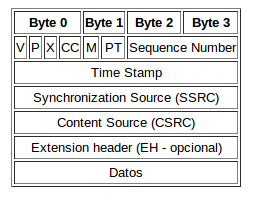
\includegraphics[width=7cm]{logos/rtp.png}
\caption{Encabezado de paquete RTP.}
\label{rtp}
\end{figure}


\begin{itemize}
\item Número de versión de RTP (V - versión number): 2 bits. La versión definida por la especificación actual es 2.

\item Relleno (P - Padding): 1 bit. Si el bit del relleno está activado, hay uno o más bytes al final del paquete que no es parte de la carga útil. El último byte del paquete indica el número de bytes de relleno. El relleno es usado por algunos algoritmos de cifrado.

\item La extensión (X - Extensión): 1 bit. Si el bit de extensión está activado, entonces el encabezado fijo es seguido por una extensión del encabezado. Este mecanismo de la extensión posibilita implementaciones para añadir información al encabezado RTP.

\item Conteo CSRC (CC): 4 bits. El número de identificadores CSRC que sigue el encabezado fijo. Si la cuenta CSRC es cero, entonces la fuente de sincronización es la fuente de la carga útil.

\item El marcador (M - Marker): 1 bit. Un bit de marcador definido por el perfil particular de media.

\item Tipo de Carga útil (PT - Payload Type): 7 bits. Un índice en una tabla del perfiles de media que describe el formato de carga útil. Los mapeos de carga útil para audio y vídeo están especificados en el RFC 1890.


\item El número de Secuencia: 16 bits. Un único número de paquete que identifica la posición de este en la secuencia de paquetes. El número del paquete es incrementado en uno para cada paquete enviado.

\item 
Sellado de tiempo: 32 bits. Refleja el instante de muestreo del primer byte en la carga útil. Varios paquetes consecutivos pueden tener el mismo sellado si son lógicamente generados en el mismo tiempo - por ejemplo, si son todo parte del mismo frame de vídeo.
\item 
SSRC: 32 bits. Identifica la fuente de sincronización. Si la cuenta CSRC es cero, entonces la fuente de carga útil es la fuente de sincronización. Si la cuenta CSRC es distinta a cero, entonces el SSRC identifica el mixer(mezclador).

\item  CSRC: 32 bits cada uno. Identifica las fuentes contribuyentes para la carga útil. El número de fuentes contribuyentes está indicado por el campo de la cuenta CSRC; Allí puede haber más de 16 fuentes contribuyentes. Si hay fuentes contribuyentes múltiples, entonces la carga útil son los datos mezclados de esas fuentes.


\item EH: El tamaño de este dato debe ser CC*32 en bits.

\item Datos: El tamaño de los datos debe ser de X *((EHL+1)*32) donde EHL es la longitud de la extensión del la cabecera en unidades de 32 bits.

\end{itemize}

\begin{verbatim}
http://en.wikipedia.org/wiki/Real-time_Transport_Protocol

http://es.wikipedia.org/wiki/User_Datagram_Protocol

\end{verbatim}



\section{Códigos de longitud variable}



\chapter{Resultados}




\section{Sistema de cifrado}

\subsection{Inversión de Bits}


Una vez que el sistema de cifrado recibe un paquete RTP, se dealiza uno  de los pasos que conforman el algoritmo propuesto:  diffuse and destroy the meaning of compressed codeword sequence and meke it impractial to predict the original codeword sequence. Para lograr esto, se propone la inversión da al menos un bit cada  $BF = F \cdot Av \cdot MEPS$ bits, donde $Av$ es el tamaño promedio de los códigos de Huffman, MEPL is the calculated Mean Average Propagation Length (MEPL) in codeword units, $Av \cdot MEPL$ es el promedio del error de propagación en bits, y $f$ is a tunable security factor with values $ \frac{1}{MEPL}  \leq f \leq \frac{3}{4}$. Para este rango de $f$, $Av \leq BF \leq Av \cdot MEPL$ esto es, al menos un bit es invertido per average Huffman codeword size ($Av$) up to $\frac{3}{4}(Av \cdot MEPL)$ bits. Esto es lo que hace nuestro system scalable secured, as $f$ gets smaller more bits are flipoed per  $BF$-bits units increasing de system security. Depending of the specific needs of the user, $f$ provides a tradeoff between security and performance.

The actual locariton $B_{i}$ del bit a ser invertido en el flujo es calculado como sigue:

\begin{equation}
B_{i}= \left( rand   \lceil \log_{2}(f \cdot Av \cdot MEPL)  \rceil \mod{BF}      \right) +1
\end{equation}

donde $rand(Numero_bits)$ is our own designed PRNG function describes in the previous section. EL argumento $ \lceil \log_{2}(f \cdot Av \cdot MEPL)  \rceil$ representa la longitud de bits of the requested random number with límites $1 \leq B_{i} \leq BF$.

The algoritm for random bit flipping in the payload P of size $P_{s}$ bytes es outlined in the following:

PONGO ALGORITMO CON LA LIBRERIA ALGORITM2e

Ahora, para lograr una mayor robustez en este paso, es importante tomar en cuenta las siguientes consideraciones:

\begin{enumerate}
\item Primer esquema. Nueva posición con referencia al inicio del bloque (gap can be considerable).

La figura ~\ref{rtp} muestra este esquema.

\begin{figure}[H]
\centering
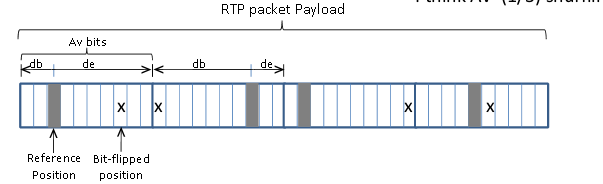
\includegraphics[width=7cm]{logos/es1.png}
\caption{Esquema 1.}
\label{eee1}
\end{figure}



\item Segundo esquema. En esta alternativa, la nueva posici[on es elegida con respecto a el $x$ previo. Esto asegura que cada uno de los bits invertidos no tienen una separación mayor de $Av$ bits. El total de bits invertidos puede ser más alto que el promedio $Av$.


La figura ~\ref{rtp} muestra el segundo esquema.

\begin{figure}[H]
\centering
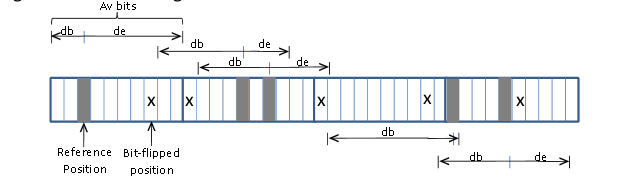
\includegraphics[width=7cm]{logos/es2.png}
\caption{Esquema 2.}
\label{eee2}
\end{figure}

A continuación se hacen algunas especificaciones para la comprensión del proceso de inversión de bits.

\begin{enumerate}
\item \textbf{db} Es el número de bits que están antes del bit de referencia.
\item \textbf{de} Es el número de bits que están después del bit de referencia.
\item \textbf{Av} El el tamaño promedio de los códigos de HUffman. Este valor se calcula por medio de la siguiente expresión:


\begin{equation}
Av = \sum_{i=1}^{N} P(C_{I})* L(C_{i}) 
\end{equation}


\end{enumerate}



\end{enumerate}



\subsection{Segment shuffling}

Después de que ha crecido el  proceso de inversión de bits, ahora, es necesario permutar los RTP-packet payload by performing an L-way shuffling. Here the payload is divided into L segmentes which are schuffled using the algorithm described below and ilustrate in figure ~\ref{shuffling}

\begin{figure}[H]
\centering
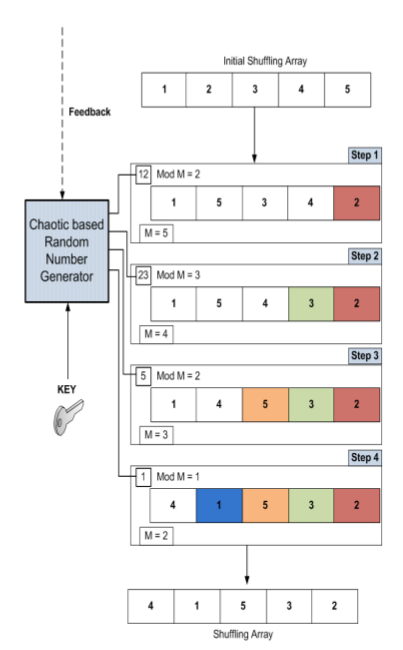
\includegraphics[width=7cm]{logos/per.png}
\caption{Esquema de permutacion.}
\label{shuffling}
\end{figure}


\subsection{Esquema robusto contra un ataque diferencial}

EL problema con el esquema de inversión de bits es que el punto de referencia del cual el número aleatorio es utilizado para invertir el bit es conocido (de el primer bit invertido la referencia es el inicio del paquete y se incrementa en Av bits), así, la idea es la siguiente: (cambiar el bit cada  $f*Av$ bits, $0 < f \leq 1$):

\begin{enumerate}
\item Elegimos una posición aleatoria ($Pos = randomChaoticNumber \mod{Av}$) de los primeros $Av$ bits in el paquete y calcular la distancia de este punto al inicio y final del bloque (en bits), ''db'' y ''de'' respectivamente.

\item Si el número aleatorio es par: $flipbitPos = (randomNumber \mod{db})$; por lo tanto $flipbitPos = Av - (randomNumber \mod{de})$. Esto es, de la posición aleatoria lanzamos una moneda (par o impar) para decidir acerca de la dirección de la inversión de bits.


\item El siguiente punto puede tomar dos direcciones, o puede ocurrir una combinación de ambos.

\begin{enumerate}
\item Ir hacia el siguiente block y repetir los pasos 1 y 2 (el inicio del siguiente blok es el nuevo punto globar de la referencia para el siguiente cálculo para la inversión del nuevo bit). EL inconveniente de este método es el espacio dejado entre bits invertidos, este puede ser más bien que $Av$ (pero como un promedio la tasa de bits invertidos es $Av$).




\item La posición del último bit invertido es el nuevo punto de referencia para el siguiente bit invertido, y se repiten los pasos 1 y 2. Para considerar la difusión del punto de referencia en la iteración actual se realiza el siguiente cálculo:

\begin{equation}
Pos = (Prev_randomChaoticNumber+new_randomChaoticNUmber) \mod{Av}
\end{equation}

el siguiente proceso es el mismo. En este esquema, los bits invertidos se encuentran aparte por no más que $Av$ bits, esto puede necesitar iteraciones adicionals al final 
\end{enumerate}
\end{enumerate}





\chapter*{Anexos}


\section*{Prueba de la Frecuencia}
La prueba consiste en medir la proporción de ceros y unos de la secuencia analizada. Se busca determinar si el número de ceros y unos en una secuencia es aproximadamente el mismo como debería ser para una secuencia verdaderamente aleatoria. La prueba evalúa que la fracción de unos  se acerce a $\frac{1}{2}$. Es importante recordar que todas las pruebas subsecuentes dependen del resultado de esta prueba.


\section*{Prueba de la Frecuencia por Bloques}
Esta prueba mide la proporción de unos en un bloque de $M$ bits, se busca determinar si la frecuencia de unos en el bloque es aproximadamente de $\frac{M}{2}$, que es el resultado esperado bajo la suposición de aleatoriedad. 

\section*{Prueba de las Corridas}
La proueba mide el número total de corridas en la secuencia, donde una corrida es una secuencia nininterrumpida de bits idénticos. Una corrida de longitud $k$ consiste de $k$ bits idénticos que está reada al inicio y al final con un bit del valor opuesto. Con esta prueba se busca demostrar si el número de coridad de ceros y unos de diversas longitudes es el que se espera para una secuencia aleatoria.

\section*{Prueba de la Corrida más Larga en un Bloque}

EL propósito de esta prueba es determinar si la longitud de la corrida más grande de unos en la secuencia probada es consistente con la longitud de la corrida más grande de unos que debería ser esperada en una secuencia aleatoria.




\section*{Prueba de la Frecuencia}
\section*{Prueba de la Frecuencia}
\section*{Prueba de la Frecuencia}
\section*{Prueba de la Frecuencia}



\addcontentsline{toc}{chapter}{Bibliography}
\bibliographystyle{alpha}
\bibliography{bibliography/bibliography}

\end{document}